\section{Présentation générale de l'application}

\subsection{Apercu général et objectif}

Le projet MazeRunner est un projet distribué destiné a générer automatiquement des recommandations musicales a partir des goûts des utilisateurs de la plateforme.
MazeRunner utilise les technologies suivantes :
\begin{itemize}
  \item Spark et GraphX pour la gestion des recommandations
  \item HDFS pour le stockage des sous-graphes permettant les recommandations
  \item RabbitMQ pour assurer la communication des différents composants
  \item neo4j pour le stockage des chansons et recommandations
  \item node.js et express.js pour l'application de démonstration.
\end{itemize}

Pour remplir la base de données neo4j, nous avons utilisé des fichiers CSV représentant les chansons interprétées dans l'emission TV "N'oubliez pas les paroles".
Nous avons ensuite créé des utilisateurs à l'image des participants au projet. Le but de cette introduction est d'avoir un regard général sur l'architecture du projet et comprendre les différentes interactions et la boucle d'exécution de MazeRunner.

\subsection{Architecture générale}

\begin{figure}[h]
    \centering
    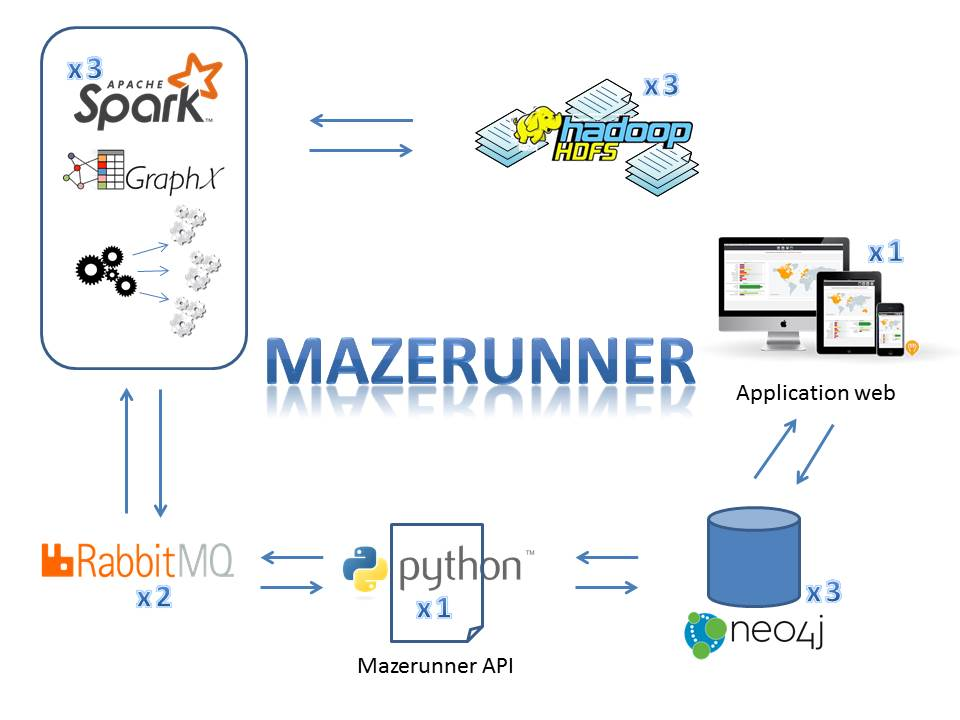
\includegraphics[scale=0.7]{pics/schema_architecture_global.jpg}
    \caption{Représentation de l'architecture générale du projet}
\end{figure}
\FloatBarrier

Comme l'indique le schéma, il y a trois machines pour les composants Spark/GraphX, trois machines pour HDFS, une machine pour l'application web, deux machines pour l'API MazeRunner, deux machines pour RabbitMQ et 3 machines pour le cluster neo4j.
Pour tous les composants sauf l'application web, le nombre de machines nous permet de garantir le fonctionnement du système malgré la panne franche d'une machine. Aussi, l'état actuel du code de l'application de démonstration ne prend pas en compte la réplication de l'API MazeRunner bien qu'effective.
Le paragraphe suivant va décrire l'exécution de la boucle permettant de générer de nouvelles recommandations ainsi que les interactions entre les composants.

\subsection{Interactions entre les composants et boucle d'exécution}

Le diagramme d'interaction permet la compréhension de la boucle d'exécution et d'expliciter comment les composants communiquent entre eux.

\begin{figure}[h]
    \centering
    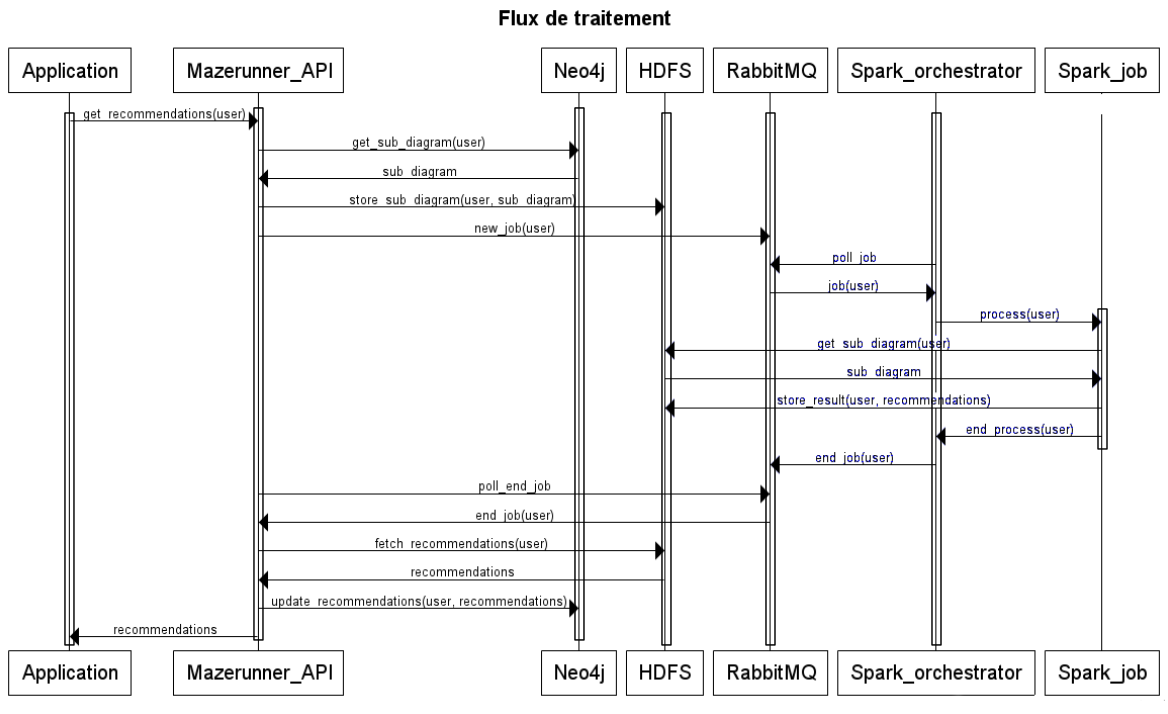
\includegraphics[scale=0.4]{pics/diagramme_interaction.png}
    \caption{Diagramme d'interaction général}
\end{figure}
\FloatBarrier

Pour accompagner le diagramme voici un descriptif de la boucle d'exécution :
\begin{itemize}
  \item L'application web demande a l'API de générer des recommandations pour l'utilisateur de l'application.
  \item L'API demande le sous-graphe correspondant a la requete a neo4j. neo4j lui envoie le sous-graphe demandé.
  \item L'API MazeRunner stocke ce sous-graphe dans HDFS a un endroit connu de Spark. Elle prévient Spark qu'un nouveau job est disponible via RabbitMQ.
  \item L'orchestrator Spark recupere le job. Le job Spark va récupérer le sous-graphe dans HDFS.
  \item Le job Spark calcule les recommandations et les stocke dans HDFS. L'orchestrator prévient l'API que le job est terminé via RabbitMQ.
  \item L'API MazeRunner vient chercher les recommandations générées dans HDFS. Il va ensuite actualiser la base de données via une requete cypher sur neo4j.
  \item L'API MazeRunner répond alors a la requete de l'application web lui indiquant que les recommandations sont disponibles sur neo4j.
  \item L'application web peut alors récupérer les recommandations calculées.
\end{itemize}
